\documentclass[../mainfile.tex]{article}
% Kopiert von kurbaniec :) 

\begin{document}
	\section{Konvergenz / Divergenz}
	\subsection*{Definition:}
	Eine Folge $a_{n}$ heißt konvergent, falls eine Zahl $a$ existiert, soo dass die folgende Bedingung erfüllt ist:\\
	Zu jedem $\epsilon > 0$ existiert ein $N \in \mathbb{N}$, so dass ab diesem Folgeglied alle Folgeglieder innerhalb der $\epsilon$-Umgebung um $a$ liegen.\\
	\\
	D.h. $\forall \epsilon > 0 \exists N \in \mathbb{N} \forall n > N: |a_{n}-a| < \epsilon$\\
	$a$ heißt Grenzwert von $a_{n}$\\
	
	$\lim\limits_{n \rightarrow \infty}{a_{n}} = a \Leftarrow $Schreibweise\\
	\\
	Ist $a_{n}$ nicht konvergent, dann heißt $a_{n}$ divergent.
	\subsection*{Erklärung:}
	\begin{figure}[h] 
		\centering
		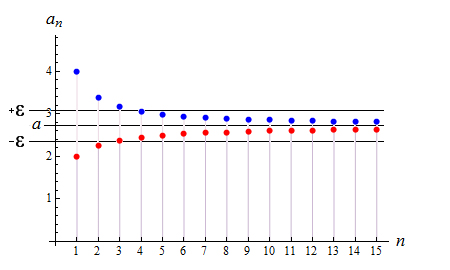
\includegraphics[width=8cm]{./swahl/img/konvergenzGraph.jpg}
		\caption{Darstellung anhand eines Graphen}
	\end{figure}
	Wichtigster Grenzwert:\\
	
	$\lim\limits_{n \rightarrow \infty}{\frac{1}{n}} = 0$\\
	\\
	Wie viele Grenzwerte kann eine Folge besitzen? $\Rightarrow$ Es kann nur einen Grenzwert geben! 
\end{document}